\section{Architektur}
\label{sec:Konzeption:Architecture}

\begin{figure}[h]
    \centering
    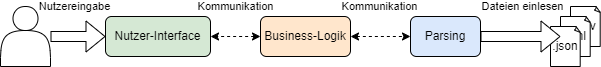
\includegraphics[width=\textwidth]{chapters/3_Konzeption/res/Architektur/class-diagramm_total.png}
    \caption{UML-Klassendiagramm der Anwendung}
    \label{fig:Konzeption:Architektur:UML-Klassendiagramm}
\end{figure}

Die Architektur der Anwendung, zu sehen in Abbildung \ref{fig:Konzeption:Architektur:UML-Klassendiagramm}, soll sich in zwei verschiedene Hauptkomponenten aufteilen, die miteinander kommunizieren: Die Business-Logik, welche sich mit dem Einlesen von Dateien und der dadurch entstehenden Generierung der Facetten auseinandersetzt und dem
Nutzer-Interface, welches die Eingabe des Nutzers annimmt, verarbeitet und an die Business-Logik weitergibt.

    \subsection{Nutzer-Interface}
    \label{subsec:Konzeption:Architektur:UI}

    \begin{figure}[th]
        \centering
        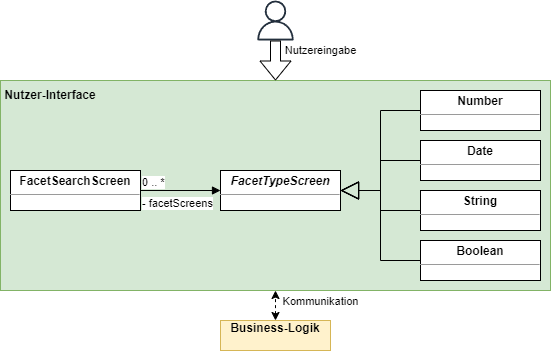
\includegraphics[width=.8\textwidth]{chapters/3_Konzeption/res/Architektur/class-diagramm_User-Interface.png}
        \caption{UML-Klassendagramm des Nutzer-Interfaces}
        \label{fig:Konzeption:Architektur:UI:UML-Klassendiagramm}
    \end{figure}

    Das in Abbildung \ref{fig:Konzeption:Architektur:UI:UML-Klassendiagramm} gezeigte Klassendiagramm stellt jeweils benötigten Komponenten für das User Interface dar, sowie deren Beziehung.

    Man sieht dass die Nutzereingabe über den ''FacetSearchScreen'' erfolgen soll.
    Er besteht aus einem oder mehreren FacetTypeScreens, welche sich auf die jeweiligen Facettentypen, besprochen in \ref{sec:Konzeption:FacetTypes}, zurückführen lassen.
    So repräsentieren NumberScreens die NumberFacetten, DateScreens die DateFacetten, StringScreens die StringFacetten und BooleanScreens die BooleanFacetten.
    Es macht aus Sich des Software Engineerings Sinn, diese Screens aufzuteilen, sodass eine bessere Übersicht, sowie Modularität herrscht.
    Falls man weitere bestimmte Screens hinzufügen oder andere entfernen möchte, so kann man das mithilfe der Vererbung sehr leicht tun.

    Um die jeweiligen Screens für deren entsprechenden Facette auswählen zu können, müssen jedoch zunächst die Facetten generiert werden, dessen Typ man prüfen kann.
    Hierzu wird die Kommunikation zwischen der Business-Logik und dem Nutzer-Interface benötigt.

    \subsection{Business-Logik}
    \label{subsec:Konzeption:Architektur:Business-Logik}

    \begin{figure}[th]
        \centering
        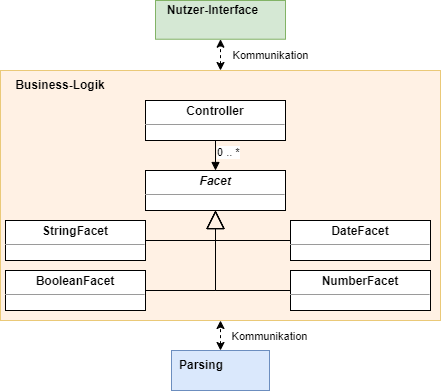
\includegraphics[width=.8\textwidth]{chapters/3_Konzeption/res/Architektur/class-diagramm_Business-Logik.png}
        \caption{UML-Klassendiagramm der Business-Logik}
        \label{fig:Konzeption:Architektur:Business-Logik:UML-Klassendiagramm}
    \end{figure}

    Das in Abbildung \ref{fig:Konzeption:Architektur:Business-Logik:UML-Klassendiagramm} gezeigte Klassendiagramm stellt die jeweiligen Komponenten für die gewollte Business-Logik dar, sowie deren Beziehungen zueinander.

    Hierbei werden die in \ref{sec:Konzeption:FacetTypes} gezeigten Facettentypen übernommen, welche alle von einer Grund-Facette erben sollen.
    Das liegt daran, dass viele Facetten die gleichen Eigenschaften übernehmen können, wie beispielsweise eine Nutzereingabe.
    Jedoch muss, wie in \ref{sec:Konzeption:FacetValue_filtering} erwähnt, auch Funktionen für jeden Facettentyp speziell geliefert werden, wodurch diese einzeln bestimmt werden müssen.

    Des Weiteren erkennt man in Abbildung \ref{fig:Konzeption:Architektur:Business-Logik:UML-Klassendiagramm} auch den Parser, welcher für das Einlesen von Dateien zuständig ist.
    Dieser Parser soll die eingelesenen Dateien dann in eine einheitliche Klasse transformieren, hier ''Document'' genannt.

    Der Controller ist dann für die Generierung der Facetten, sowie weitere logische Schritte notwendig.
    Hierfür benötigt er die ''Document''-Klasse, sodass er anhand der Objekte eben jene Facetten generieren kann.

    \subsection{Parsing}
    \label{subsec:Konzeption:Architektur:Parsing}
    
    \begin{figure}[h]
        \centering
        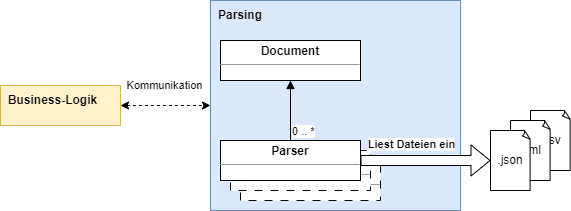
\includegraphics[width=\textwidth]{chapters/3_Konzeption/res/Architektur/class-diagramm_Parsing.png}
        \caption{UML-Klassendiagramm für das Parsing verschiedener Datenformate}
        \label{fig:Konzeption:Architektur:Parsing:Klassendiagramm}
    \end{figure}
    
    In Abbildung \ref{fig:Konzeption:Architektur:Parsing:Klassendiagramm} sind unterschiedliche Parser zu sehen, die ihren jeweiligen Datei-Typen in eine eigene Klasse transformieren.
    Diese Dokumenten-Klasse soll zur Generalisierung der verschiedenen Datenstrukturen verwendet werden, wodurch eine Modularität erzeugt wird, die es zulässt verschiedene Parser für ihre jeweiligen Datei-Strukturen zu entwickeln.
    Hierbei sollen die Dokumente gelesen, verarbeitet und als Dokumenten-Objekte abgespeichert werden.
    Die Business-Logik soll dann auf diese Objekte zugreifen, um aus ihnen die Facetten zu generieren.
    
    So soll es beispielsweise einen JSON-Parser für ''.json''-Dokumente, einen XML-Parser für ''.xml''-Dokumente usw. geben, die diese Dokumenten-Typen dann in ein Dokumenten-Objekt transformieren, mit dem gearbeitet werden kann.
    Die dadurch erzeugte Modularität lässt ein einfaches Hinzufügen oder Entfernen verschiedener Dokumentenstrukturen zu.